\documentclass[11pt,twocolumn,letterpaper]{article}

\usepackage{cvpr}
\usepackage{times}
\usepackage{epsfig}
\usepackage{graphicx}
\usepackage{amsmath}
\usepackage{amssymb}

%used for drawing flow chart
\usepackage{tikz}
\usetikzlibrary{shapes,arrows,positioning,fit,calc}
\usepackage{subfig}

% Include other packages here, before hyperref.

% If you comment hyperref and then uncomment it, you should delete
% egpaper.aux before re-running latex.  (Or just hit 'q' on the first latex
% run, let it finish, and you should be clear).
\usepackage[breaklinks=true,bookmarks=false]{hyperref}

\cvprfinalcopy % *** Uncomment this line for the final submission

\def\cvprPaperID{****} % *** Enter the CVPR Paper ID here
\def\httilde{\mbox{\tt\raisebox{-.5ex}{\symbol{126}}}}

% Pages are numbered in submission mode, and unnumbered in camera-ready
%\ifcvprfinal\pagestyle{empty}\fi
\begin{document}

\title{Recurrent Human Pose Estimation \\ \small CS231A Project}
\author{Matthew Chen\\
  \small \vspace{-2mm} Department of Computer Science\\
  \small \vspace{-2mm} Stanford University\\
  \small mcc17@stanford.edu
  \and
  Melvin Low\\
  \small \vspace{-2mm} Department of Computer Science\\
  \small \vspace{-2mm} Stanford University\\
  \small mwlow@stanford.edu}

\date{}
\maketitle
\newcommand{\argmin}{\operatornamewithlimits{arg\,min}}
\newcommand{\argmax}{\operatornamewithlimits{arg\,max}}
\section{Introduction}

Human pose estimation is the task of estimating the joint locations of one or
multiple people within an image. It is a core challenge in computer vision because
it forms the foundation of more complex tasks such as activity recognition
and motion planning. For example, joint locations have been used to supplement
other visual features to determine the trajectory of a person through a sequence
of video frames.

In the past, the leading techniques for pose estimation were the deformable
parts model and its variants. These approaches used convolutions of fast
part detectors over the input image to generate a coherent 
joint configuration \cite{felzenszwalb2010object}.
More recently, deep learning techniques such as convolutional neural networks
as well as optimization methods such as mixed integer programs have 
achieved state of the art results, for detecting both single and multiple people.

From a probabilistic perspective, pose estimation is the task of finding
a joint configuration of $n$ joints, $y_1, y_2,..., y_n$, given a source image $x$, i.e.
$\argmax_{y_1,...,y_n} p(y_1,...y_n|x)$. Several state of the art methods
have attempted to calculate this directly with a convolutional neural net. While
this has worked very well, the natural dependencies between human joints suggest
that explicitly modeling these dependencies may give a boost in performance.
This corresponds to calculating 
$$\argmax_{y_i} p(y_i | y_{i-1}, y_{i-2},...,y_1, x), i = 1, 2,...,n$$\textemdash generating 
the joints one at a time in sequence. 
This paper investigates this approach. We
use a recurent network architecture, which is particularly well suited for
capturing sequence information. Preliminary results show that the recurrent
approach unfortunately performs much worse than the straightforward convolutional one. It
seems to enforce joint relationships too strongly and thus tends toward the most common
pose in the dataset.

\section{Previous Work}

Prior to the widespread use of neural networks in computer vision, classic approaches were applied to the problem of pose estimation. These approaches generally took the form of expressing the body as a graphical model and encoding priors on the likely configurations of the parts \cite{felzenszwalb2005pictorial}. A joint objective would then be optimized which accounted for both the match score from a part detector and the likelihood of the resulting configuration. These models, however, suffer in terms of computational tractability as they involve inference over a graphical model. Many of the techniques deployed to improve the tractability come with costs to the expressiveness of such models\cite{yang2011articulated}.

DeepPose was one of the first papers to deploy deep networks for this problem. The authors formulated the problem as a regression task. In their model the 
joint coordinates were predicted directly from a regression layer of a convolutional neural network (CNN). Due to the need to downsize the original image to fit the fixed CNN input size of 224 by 224 they used a cascade of CNN classifiers \cite{toshev2014deeppose}, each cropping the picture centred around the previous prediction at a higher resolution, to further refine their pose estimates. One issue with this approach is that the errors from previous mistakes can propagate into future decisions as each choice involves a crop of the image and thus limits the possible domain of solutions.

\cite{carreira2015human} similarly use a CNN to predict joint coordinates but add a iterative feedback mechanism where an initial pose is refined at every timestep given the image and the previous estimate. They accomplish this by defining an error function over joint offsets which measures the residual estimate error and learn a model to minimize this objective. An advantage of such an approach is that each timestep can get a better estimate of the joint distribution of the body pose given the previous estimate, incorporating some of the dependencies which exist between them. This idea of iterative refinement has been broadly adapted in many of the subsequent works. The methodology seems to build upon recent work on efficiently training deep networks by using residuals \cite{he2015deep}.

A feedback mechanism is used in \cite{haque2016viewpoint} to model pose error in 3D images using a recurrent neural network (RNN). They find that using an RNN is able to improve performance by taking into account error dependencies across refinement steps. However, we have not found much in literature regarding a recurrent approach to directly model the joints.

Another notable approach, DeepCut, formulated the problem as an integer linear program and solves a global optimization problem \cite{pishchulin2015deepcut}. The problem addresses the multi-person pose estimation which generalizes the single person task which we focus on in this paper. Their approach involves inference over a probabilistic model in which they use part detectors as unary factors and joint part dependencies as binary factors. In this light, it builds upon some of the previous ideas used in deformable parts models. However they use more expressive parts detectors, an adaptation of recent detection work \cite{ren2015faster}, and a global objective function.

One limitation of using a standard CNN based model is that information, which can be used for fine grained localization, can be lost in the pooling layers of the network. This problem was addressed in Deep Pose with the cascade of networks, however this approach propagated errors from previous decisions.Two recent papers are able to achieve new state of the art results by addressing these limitations in their models. In Pose Machines, the authors take a multi-stage approach where they extract features from a local region in the image in one stage and then incorporate more global features in the latter stages \cite{wei2016convolutional}. Each stage is trained with using intermediate supervision and is able to iteratively refine the initial joint estimates with more information.

Similarly in Stacked Hourglass Networks, the authors propose a architecture which involves extracting features from images at different scales. These features are then concatenated with a deconvolution stage, creating an hourglass shape architecture \cite{newell2016stacked}. By running the network across scales the architecture is theoretically able to incorporate global and local information into its estimates. Furthermore the stacking of multiple hourglasses can be seen as another form of iterative refinement.

%TODO : add a paragraph about attention models since we include this in our paper
%TODO : relate back to what we are doing for this paper

\section{Dataset}


We used the MPII human pose estimation dataset, which is composed of 25,000 RGB 
images annotated with over 40,000 human poses \cite{andriluka20142d}. The images were collected by sampling 3,913 videos from Youtube in various frames, which are at least 5 seconds apart, and filtering images which contained people. The annotations were obtained via crowd sourcing on Amazon Mechanical Turk and take the form of pixels coordinates 
corresponding to 16 joints for a given person in an image. A given image
may contain multiple people, so we centered and cropped each image around a single person with some padding around their joint locations.


\section{Methodology}

We hypothesize that estimating joint locations sequentially will be able to better capture the dependency between joint locations since we explicitly condition on previous joint decisions. We choose to use a recurrent neural network model because it is able to express dependencies across sequences. Such models are common in natural language tasks which are naturally modelled as sequences. To test this hypothesis we choose our comparison baseline model to be a generic CNN which regresses all joint locations in one pass. This is similar to the method proposed in DeepPose, however we do not implement their cascade of network classifiers so we can isolate the effects of the sequence modelling without the added effect of refinement through higher resolution. For our experimental model we use a RNN whose inputs are feature which were extracted from the last convolutional layers of the CNN used for the base model. Comparing the two would thus show the difference in performance based on modelling the pose as a sequence. Full details on the models used are provided below.


\subsection{CNN Base Architecture}

\begin{table}
\begin{center}
\begin{tabular}{| c | c | c |}
\hline
Section & Type & Parameters\\
\hline\hline
Layer 1 & conv3-64 & 1,728\\
&conv3-64 & 36,864\\
&maxpool & 0\\
Layer 2&conv3-128 & 73,728\\
&conv3-128 & 147,456\\
&maxpool & 0\\
Layer 3&conv3-256 & 294,912\\
&conv3-256 & 589,824\\
&conv3-256 & 589,824\\
&maxpool & 0\\
Layer 4&conv3-512 & 1,179,648\\
&conv3-512 & 2,359,296\\
&conv3-512 & 2,359,296\\
&maxpool & 0\\
Layer 5&conv3-512 & 2,359,296\\
&conv3-512 & 2,359,296\\
&conv3-512 & 2,359,296\\
&maxpool & 0\\
Layer 6&fc-4096 & 102,760,448\\
Layer 7&fc-4096 & 16,777,216\\
&fc-19 & 77,824\\
&softmax & 0\\
\hline
Total & & 134,325,952\\
\hline
\end{tabular}
\end{center}
\caption{VGGNet architecture and number of parameters}
\label{vgg_arch}
\end{table}

%TODO : Elaborate on this

We implemented a CNN based off of VGG16 as our base model \cite{simonyan2014very}. 
VGG16 consists of a stack of convolutional layers followed by two fully connected layers.
We modified the network
by adding batch normalization layers after each nonlinearity in order to improve training.
The output of the fully connected layers was a 32 dimensional vector, corresponding to
the $(x, y)$ coordinates of 16 joints.

\subsection{CNN-RNN Architecture}

%define flowchart elements
\tikzstyle{pipe} = [rectangle, draw, fill=orange!30, rounded corners, text width=4.5em, text height=2em, text badly centered, node distance=7em, inner sep=0pt]
\tikzstyle{line} = [draw, -latex']


\begin{figure}
\begin{center}
\begin{tikzpicture}
\node[pipe] (img) {Image};
\node[pipe, right = 3mm of img] (CNN) {CNN};
\node[pipe, right of=CNN] (lstm3) {LSTM};
\node[pipe, above = 3mm of lstm3] (lstm2) {LSTM};
\node[pipe, above = 3mm of lstm2] (lstm1) {LSTM};

\node[pipe, right = 4mm of lstm1] (head) {Head};
\node[pipe, right = 4mm of lstm2] (sh1) {Shoulder1};
\node[pipe, right = 4mm of lstm3] (sh2) {Shoulder2};


\path[line] (img)--(CNN);
\path[line] (CNN)--(lstm1);
\path[line] (CNN)--(lstm2);
\path[line] (CNN)--(lstm3);
\path[line] (lstm1)--(lstm2);
\path[line] (lstm2)--(lstm3);

\path[line] (lstm1)--(head);
\path[line] (lstm2)--(sh1);
\path[line] (lstm3)--(sh2);
\end{tikzpicture}
\label{model_diag}
\caption{CNN-RNN architecture. A CNN is used to extract features from each image, which are
then fed into an LSTM. The LSTM produces joint coordinates in pixel space.}
\label{fig:lstm_diag}
\end{center}
\end{figure}

We used the same base architecture to produce the initial hidden state and input
to the RNN. A long short-term memory (LSTM) architecture was used for the RNN. The LSTM
augments the traditional RNN formulation with a cell state, which allows
gradients to flow additively through the network instead of multiplicatively.
Concretely, at each timestep, the LSTM takes $x_t$, $h_{t-1}$,
$c_{t-1}$ and produces $h_t$, $c_t$ via the following calculations:

\begin{align*}
    i_t &= \sigma(W^ix_t + U^ih_{t-1} + b^i)\\
    f_t &= \sigma(W^fx_t + U^fh_{t-1} + b^f)\\
    o_t &= \sigma(W^ox_t + U^oh_{t-1} + b^o)\\
    g_t &= \text{tanh}(W^gx_t + U^gh_{t-1} + b^g)\\
    c_t &= f_t \odot c_{t-1} + i_t \odot g_t\\
    h_t &= o_t \odot \text{tanh}(c_t)
\end{align*}

where $i_t$, $f_t$, $o_t$ are the input, forget, and output gates. This structure
improves gradient flow and has resulted in LSTMs being used to great success in recent literature
for a wide variety of tasks. 

We used two stacked LSTMs with a hidden state size of 128 and 16 timesteps. At each timestep,
the hidden state of the LSTMs was projected into a two dimensional vector, which 
corresponded to the location of a single joint in the image (hence 16 timesteps for 16 joints).

\subsection{LSTM with Attention}

We additionally added soft attention to our CNN-RNN model. Soft attention
was introduced by Xu et al. \cite{xu2015show} and described a method to ``guide''
the focus of the recurrent neural network through the input image, over time. The
mechanism attempted to relieve the feature encoder (a convolutional neural network in
both our work and Xu et al.) of the need to compress the entire image into a single
output vector. In order to implement attention, we made the following changes:

\begin{itemize}
    \item We removed the two fully connected layers from our CNN, as suggested by
        Xu et al. Instead, we take the output of the last convolutional layer
        as input to the recurrent network. We call this output
        the \textit{annotation vectors} or \textit{annots},
        with dimensions $(w*h, c)$ for a single image. $c$ is the number of channels of
        the last convolutional filter, and $w$ and $h$ are the width and height of
        the image after passing through multiple max-pooling layers. In our case,
        $w = h = 14$ and $c = 512$. Thus we have 196 row vectors of size 512 each.

    \item At every timestep $t$, we calculate $$\alpha = MLP(h_{t-1}, annots)$$,
        where MLP is a multiplayer perceptron and $h_{t-1}$ is the hidden state of the
        LSTM from the previous timestep. $\alpha$ is a single vector of dimension $wh$, or
        196 in our case. The initial state of the LSTM is the mean of the annotation vectors.

    \item We calculate the next input to the LSTM as the weighted sum of the annotation
        vectors, $\alpha * annots$. 
\end{itemize}



%TODO : A hidden layer is inserted prior to the regression layer
%TODO : Talk about size of hidden layers, state/cell initializations - how this could have affected the results

\subsection{Training}

%TODO : a brief two points about what adam is compared to other optimizers/advantages would be helpful
We used $l_2$ loss aggregated over all timesteps. 
The stochastic optimizer was Adam, which is a recent optimizer which was shown empirically
to be 
faster than stochastic gradient descent. The learning
rate was set initially to 0.001, and was reduced by a factor of 2 every 1000 batch iterations.
The model was implemented using TensorFlow and took one day to train on a Nvidia GTX 980 Ti.

\subsection{Evaluation}

%TODO : previous measures of PCK - and how we got to the current measure. Strengths and limitations ( previous measure are PCP and PCKh)

To compare our results to previous works we use the standard percentage of correct keypoints (PCKh) measure. The h denotes that the measure is normalized by the length of the head in each image. This measure is calculated by counting the percentage of correct localizations for a given part across all images. A estimate is classified as correct if it falls within a certain distance of the ground truth annotation. That distance is defined to be half the length of the persons head in a given image.

\section{Results}

\begin{table*}
\centering
\begin{tabular}{l l l l l l l l l}
\hline \hline
Method & Head & Shoulder & Elbow & Wrist & Hip & Knee & Ankle & Total\\
\hline
Iterative Error\cite{carreira2015human} & 95.7 & 91.7 & 81.7 & 72.4 & 82.8 & 73.2 & 66.4 & 81.3\\
DeepCut\cite{pishchulin2015deepcut} & 94.1 & 90.2 & 83.4 & 77.3 & 82.6 & 75.7 & 68.6 & 82.4\\
Pose Machines\cite{wei2016convolutional} & 97.7 & 94.5 & 88.3 & 83.4 & 87.9 & 81.9 & 78.3 & 87.9\\
Stacked Hourglass\cite{newell2016stacked} & 97.6 & 95.4 & 90.0 & 85.2 & 88.7 & 85.0 & 80.6 & 89.4\\
\hline
Our Base Model & 52.0 & 40.6 & 22.5 & 16.8 & 31.7 & 21.2 & 16.0 & 32.8\\
Our LSTM Model & 39.2 & 25.2 & 12.2 & 9.7 & 18.7 & 16.6 & 7.5 & 21.5 \\
\hline \hline
\end{tabular}
\caption{Model Performance Comparison (PCKh)}
\end{table*}

\begin{figure}[!ht]
\begin{center}
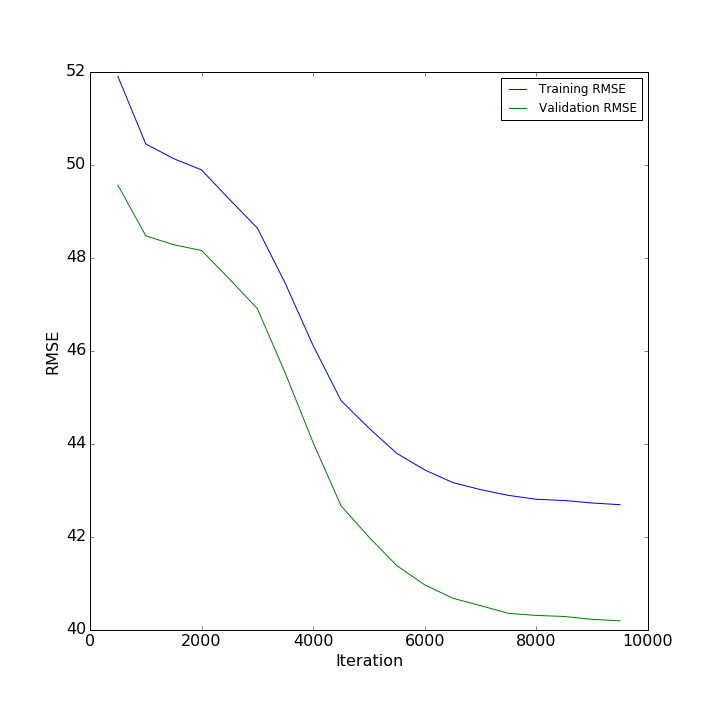
\includegraphics[scale=0.35]{images/base_loss}
\end{center}
\caption{Training and validation RMSE over time for the CNN base model.}
\label{fig:1}

\end{figure}

\begin{figure}[!ht]
\begin{center}
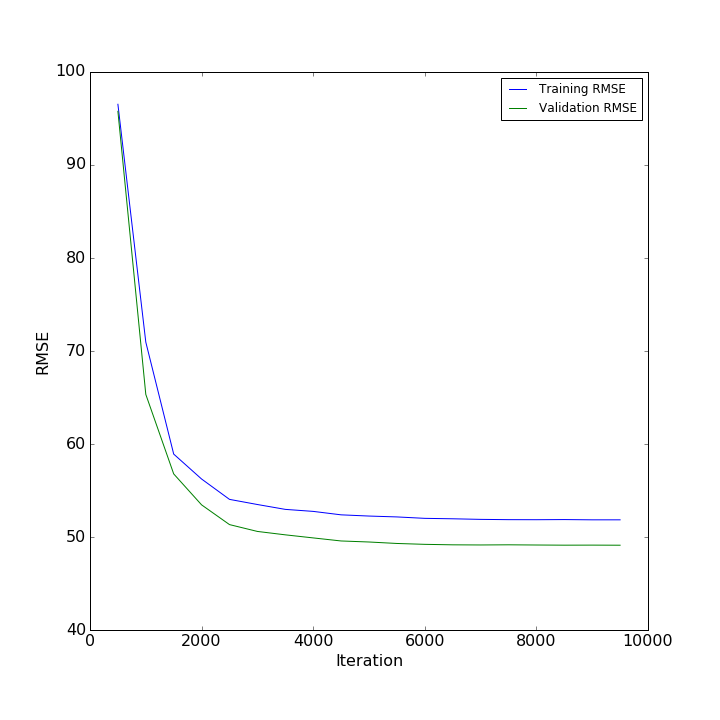
\includegraphics[scale=0.35]{images/rnn_loss}
\end{center}
\caption{Training and validation RMSE over time for the RNN-CNN model.}
\label{fig:2}
\end{figure}

The CNN base architecture performed much better than the CNN-RNN one. 
The root mean squared errors of both models can be seen in figures \ref{fig:1} and \ref{fig:2}.
Sample pictures for both models are provided in figures \ref{fig:base_images} and \ref{fig:rnn_images}. Finally, PCKh measures and comparisons are provided in table 1. 

Adding attention to the LSTM did not, unfortunately, improve or change its performance.
Thus, we did not include the attention results for sake of conciseness, and the results
shown in the following sections are for the simple LSTM model.

Validation loss and error rates improved with both models. However, only the CNN seemed
to be learning the correct pose effectively. The CNN-RNN, on the other hand, did not 
perform well. It seemed to be producing the same pose regardless of the input image.


\begin{figure}
\begin{tabular}{cc}
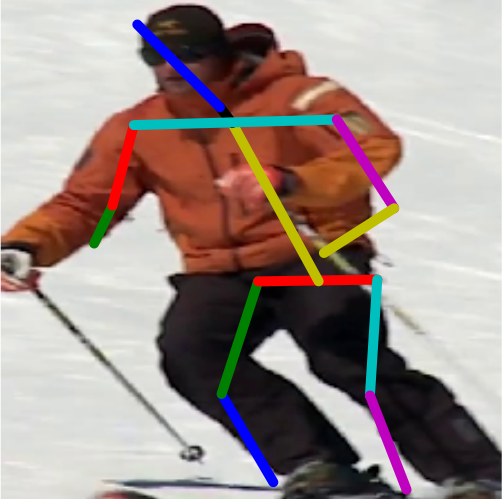
\includegraphics[width=40mm]{images/base_1}
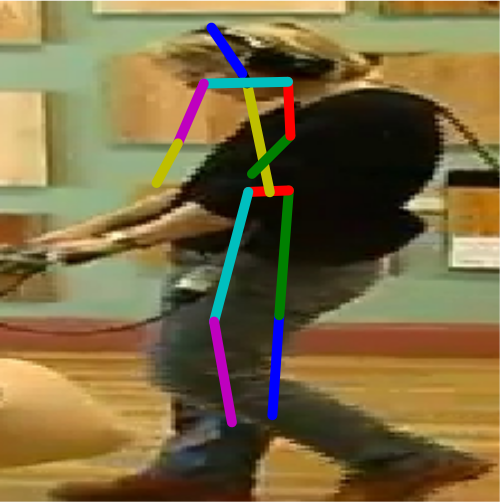
\includegraphics[width=40mm]{images/base_2}\\
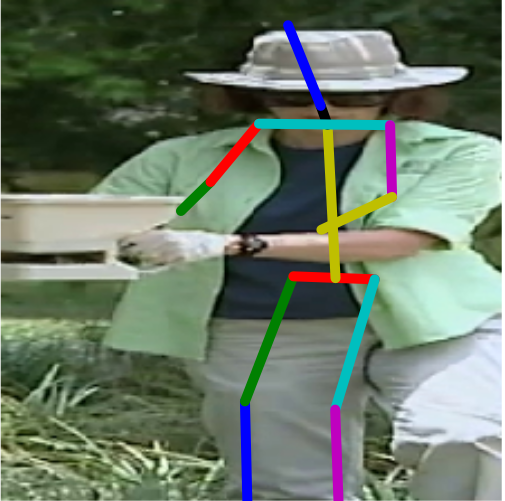
\includegraphics[width=40mm]{images/base_3}
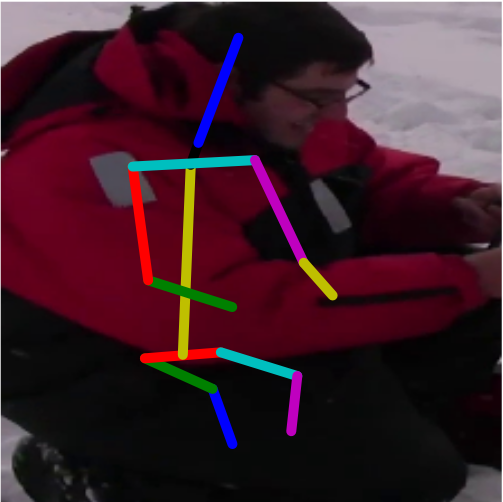
\includegraphics[width=40mm]{images/base_4}\\
\end{tabular}
\caption{Sample predictions for the CNN base model. The model seems to be learning
    effectively.}
\label{fig:base_images}
\end{figure}

\begin{figure}
\begin{tabular}{cc}
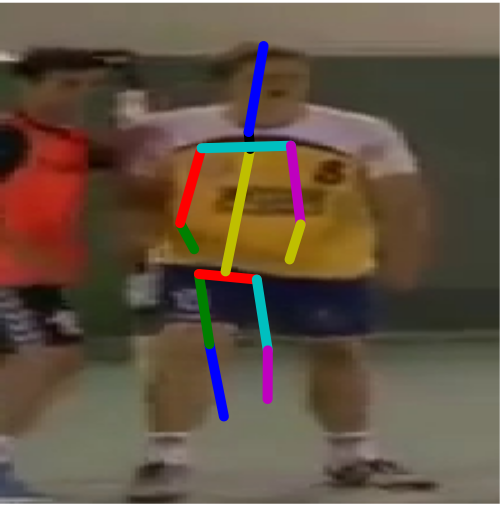
\includegraphics[width=40mm]{images/rnn_1}
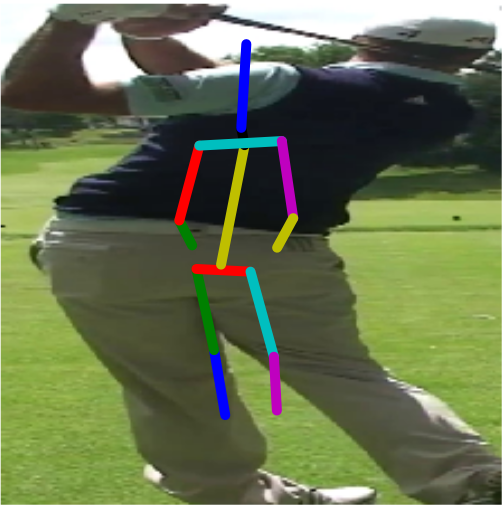
\includegraphics[width=40mm]{images/rnn_2}\\
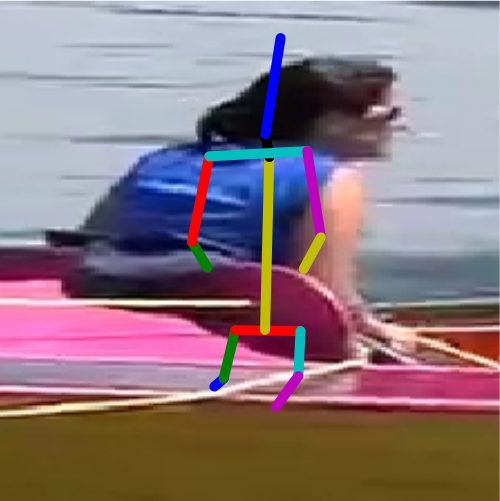
\includegraphics[width=40mm]{images/rnn_3}
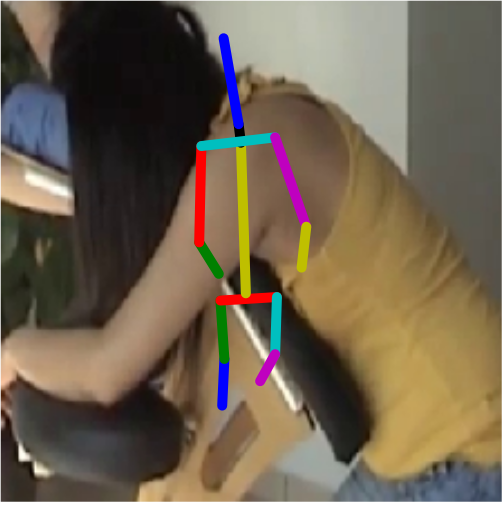
\includegraphics[width=40mm]{images/rnn_4}\\
\end{tabular}
\caption{Sample predictions for the CNN-RNN model. The estimated poses seem to be shifting 
    slightly toward ground truth, but seem to contain noticeable ``inertia.''}
\label{fig:rnn_images}
\end{figure}

\section{Discussion}

We suspect that the recurrent network regressed toward the most common
pose in the dataset. This might occur, for example, if the RNN had not
learned to fully utilize the output of the CNN or the CNN was not
well-trained, and thus the model was calculating:

$$\argmax_{y_i} p(y_i | y_{i-1}, y_{i-2},...,y_1), i = 1, 2,...,n$$

instead of:

$$\argmax_{y_i} p(y_i | y_{i-1}, y_{i-2},...,y_1, x), i = 1, 2,...,n$$.

This would be problematic because it may be the case that knowing $y_1$ alone
may be insufficient to estimate the correct $y_2$. In this case, estimating
the most common pose would make sense. Having a larger training 
set may have alleviated this problem. We also
suspect that errors compounded through time in the recurrent network. Specifically,
if $\argmax_{y_2} p(y_2 | y_{1}, x)$ is calculated incorrectly, then it
is likely that $\argmax_{y_3} p(y_3 | y_{2}, y_{1}, x)$ would 
also be calculated incorrectly. The base model did not explicitly
model these conditional probabilities so it would not suffer from this problem.

Another possible explantion for why the LSTM performed poorly is that 
modeling joints as a sequence placed too many constraints on the model.
In other words, the recurrent formulation of the problem was incorrect. 
This might explain why adding attention did not improve the performance
of the LSTM. Attention gives more information to the recurrent network,
but if a recurrent structure was incorrect to begin with, then it would not
help.


\section{Conclusion}

In this project, we investigated the possibility of modelling pose estimation
as a sequence task. We tested this hypothesis via use of a convolutional
network linked to a recurrent one. For comparison, we also
tested just the convolutional network on the same task. Our preliminary results show that 
the CNN-RNN performed worse than the CNN. 
Furthermore, adding attention did not improve the result of the
CNN-RNN.

%TODO : include potential for future work


\nocite{*}
\bibliographystyle{ieee}
\bibliography{final}

\end{document}
